\section{Design}

\begin{figure*}[h]
    \centering
    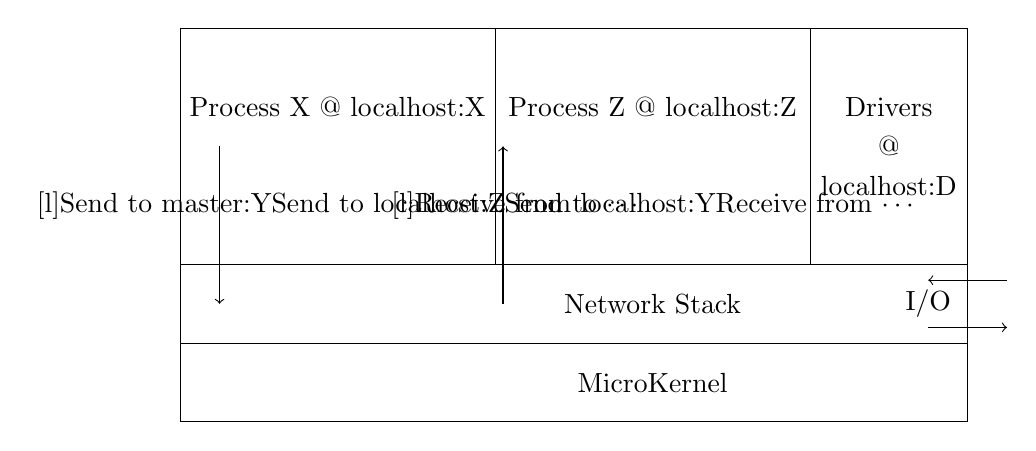
\begin{tikzpicture}

        \begin{scope}[shift={(1,1)},local bounding box=IoTOS]
            \draw (0,0) rectangle (10, 5);
            \draw (0,1) rectangle (10, 2);
            \draw (0,2) rectangle (4, 5);
            \draw (4, 2) rectangle (8, 5);
            
            \node at (6, 0.5) {MicroKernel};
            \node at (6, 1.5) {Network Stack};
            
            \node at (2, 4) {Process X @ localhost:X};
            \node at (2, 2.75) {\makecell[l]{Send to master:Y \\ Send to localhost:Z  \\ Send to $\cdots$}};
            \draw[->] (0.5, 3.5) -- (0.5, 1.5);

            \node at (6, 2.75) {\makecell[l]{Receive from localhost:Y  \\ Receive from $\cdots$}};
            \draw[->] (4.1, 1.5) -- (4.1, 3.5);

            \node at (6, 4) { Process Z @ localhost:Z };
            \node at (9, 4) { Drivers };
            \node at (9, 3.5) { @ };
            \node at (9, 3) { localhost:D };

            \node at (9.5, 1.5) {I/O};
            \draw[->] (9.5, 1.2) -- (10.5, 1.2);
            \draw[->] (10.5, 1.8) -- (9.5, 1.8);
            
        \end{scope}
        
        IoTOS
\end{tikzpicture}
\end{figure*}